\documentclass[tikz,border=1pt]{standalone}
\usepackage{fontspec}
\setmainfont{Times New Roman}

\usetikzlibrary{positioning,arrows.meta}

% Pure black-and-white palette for print
\begin{document}
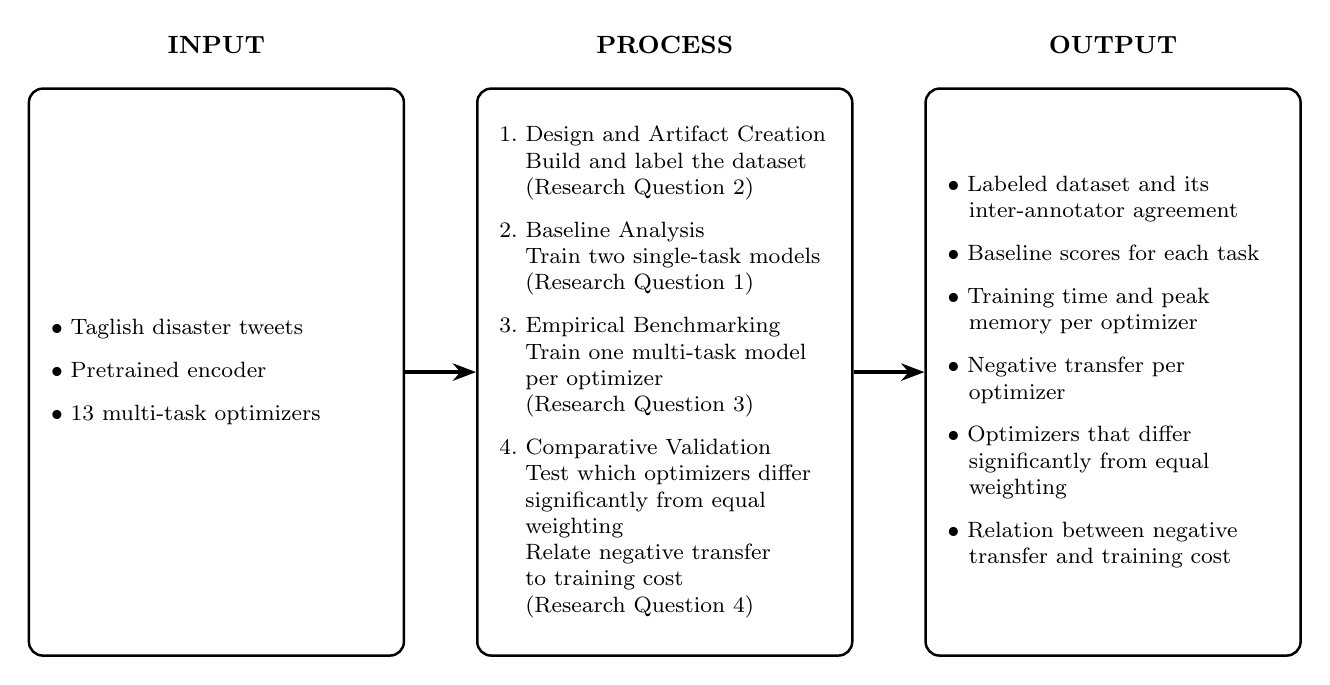
\begin{tikzpicture}[
    font=\small,
    >=Stealth,
    iobox/.style={draw=black, rounded corners=5pt, align=left,
        text width=4.2cm, minimum height=7.2cm, inner sep=8pt,
        font=\footnotesize, line width=0.9pt},
    head/.style={font=\small\bfseries},
    bigarrow/.style={->, very thick}
]

    \node[iobox] (input) {
        $\bullet$~Taglish disaster tweets\\[6pt]
        $\bullet$~Pretrained encoder\\[6pt]
        $\bullet$~13 multi-task optimizers
    };

    \node[iobox, right=0.9cm of input] (process) {
        1.~Design and Artifact Creation\\
        \hspace*{1.1em}Build and label the dataset\\
        \hspace*{1.1em}(Research Question 2)\\[6pt]
        2.~Baseline Analysis\\
        \hspace*{1.1em}Train two single-task models\\
        \hspace*{1.1em}(Research Question 1)\\[6pt]
        3.~Empirical Benchmarking\\
        \hspace*{1.1em}Train one multi-task model\\
        \hspace*{1.1em}per optimizer\\
        \hspace*{1.1em}(Research Question 3)\\[6pt]
        4.~Comparative Validation\\
        \hspace*{1.1em}Test which optimizers differ\\
        \hspace*{1.1em}significantly from equal\\
        \hspace*{1.1em}weighting\\
        \hspace*{1.1em}Relate negative transfer\\
        \hspace*{1.1em}to training cost\\
        \hspace*{1.1em}(Research Question 4)
    };

    \node[iobox, right=0.9cm of process] (output) {
        $\bullet$~Labeled dataset and its\\
        \hspace*{0.9em}inter-annotator agreement\\[6pt]
        $\bullet$~Baseline scores for each task\\[6pt]
        $\bullet$~Training time and peak\\
        \hspace*{0.9em}memory per optimizer\\[6pt]
        $\bullet$~Negative transfer per\\
        \hspace*{0.9em}optimizer\\[6pt]
        $\bullet$~Optimizers that differ\\
        \hspace*{0.9em}significantly from equal\\
        \hspace*{0.9em}weighting\\[6pt]
        $\bullet$~Relation between negative\\
        \hspace*{0.9em}transfer and training cost
    };

    \node[head, above=0.3cm of input] {INPUT};
    \node[head, above=0.3cm of process] {PROCESS};
    \node[head, above=0.3cm of output] {OUTPUT};

    \draw[bigarrow] (input) -- (process);
    \draw[bigarrow] (process) -- (output);

\end{tikzpicture}
\end{document}
